% Options for packages loaded elsewhere
\PassOptionsToPackage{unicode}{hyperref}
\PassOptionsToPackage{hyphens}{url}
%
\documentclass[
]{article}
\usepackage{lmodern}
\usepackage{amssymb,amsmath}
\usepackage{ifxetex,ifluatex}
\ifnum 0\ifxetex 1\fi\ifluatex 1\fi=0 % if pdftex
  \usepackage[T1]{fontenc}
  \usepackage[utf8]{inputenc}
  \usepackage{textcomp} % provide euro and other symbols
\else % if luatex or xetex
  \usepackage{unicode-math}
  \defaultfontfeatures{Scale=MatchLowercase}
  \defaultfontfeatures[\rmfamily]{Ligatures=TeX,Scale=1}
\fi
% Use upquote if available, for straight quotes in verbatim environments
\IfFileExists{upquote.sty}{\usepackage{upquote}}{}
\IfFileExists{microtype.sty}{% use microtype if available
  \usepackage[]{microtype}
  \UseMicrotypeSet[protrusion]{basicmath} % disable protrusion for tt fonts
}{}
\makeatletter
\@ifundefined{KOMAClassName}{% if non-KOMA class
  \IfFileExists{parskip.sty}{%
    \usepackage{parskip}
  }{% else
    \setlength{\parindent}{0pt}
    \setlength{\parskip}{6pt plus 2pt minus 1pt}}
}{% if KOMA class
  \KOMAoptions{parskip=half}}
\makeatother
\usepackage{xcolor}
\IfFileExists{xurl.sty}{\usepackage{xurl}}{} % add URL line breaks if available
\IfFileExists{bookmark.sty}{\usepackage{bookmark}}{\usepackage{hyperref}}
\hypersetup{
  pdftitle={R Markdown Output},
  hidelinks,
  pdfcreator={LaTeX via pandoc}}
\urlstyle{same} % disable monospaced font for URLs
\usepackage[margin=1in]{geometry}
\usepackage{color}
\usepackage{fancyvrb}
\newcommand{\VerbBar}{|}
\newcommand{\VERB}{\Verb[commandchars=\\\{\}]}
\DefineVerbatimEnvironment{Highlighting}{Verbatim}{commandchars=\\\{\}}
% Add ',fontsize=\small' for more characters per line
\usepackage{framed}
\definecolor{shadecolor}{RGB}{248,248,248}
\newenvironment{Shaded}{\begin{snugshade}}{\end{snugshade}}
\newcommand{\AlertTok}[1]{\textcolor[rgb]{0.94,0.16,0.16}{#1}}
\newcommand{\AnnotationTok}[1]{\textcolor[rgb]{0.56,0.35,0.01}{\textbf{\textit{#1}}}}
\newcommand{\AttributeTok}[1]{\textcolor[rgb]{0.77,0.63,0.00}{#1}}
\newcommand{\BaseNTok}[1]{\textcolor[rgb]{0.00,0.00,0.81}{#1}}
\newcommand{\BuiltInTok}[1]{#1}
\newcommand{\CharTok}[1]{\textcolor[rgb]{0.31,0.60,0.02}{#1}}
\newcommand{\CommentTok}[1]{\textcolor[rgb]{0.56,0.35,0.01}{\textit{#1}}}
\newcommand{\CommentVarTok}[1]{\textcolor[rgb]{0.56,0.35,0.01}{\textbf{\textit{#1}}}}
\newcommand{\ConstantTok}[1]{\textcolor[rgb]{0.00,0.00,0.00}{#1}}
\newcommand{\ControlFlowTok}[1]{\textcolor[rgb]{0.13,0.29,0.53}{\textbf{#1}}}
\newcommand{\DataTypeTok}[1]{\textcolor[rgb]{0.13,0.29,0.53}{#1}}
\newcommand{\DecValTok}[1]{\textcolor[rgb]{0.00,0.00,0.81}{#1}}
\newcommand{\DocumentationTok}[1]{\textcolor[rgb]{0.56,0.35,0.01}{\textbf{\textit{#1}}}}
\newcommand{\ErrorTok}[1]{\textcolor[rgb]{0.64,0.00,0.00}{\textbf{#1}}}
\newcommand{\ExtensionTok}[1]{#1}
\newcommand{\FloatTok}[1]{\textcolor[rgb]{0.00,0.00,0.81}{#1}}
\newcommand{\FunctionTok}[1]{\textcolor[rgb]{0.00,0.00,0.00}{#1}}
\newcommand{\ImportTok}[1]{#1}
\newcommand{\InformationTok}[1]{\textcolor[rgb]{0.56,0.35,0.01}{\textbf{\textit{#1}}}}
\newcommand{\KeywordTok}[1]{\textcolor[rgb]{0.13,0.29,0.53}{\textbf{#1}}}
\newcommand{\NormalTok}[1]{#1}
\newcommand{\OperatorTok}[1]{\textcolor[rgb]{0.81,0.36,0.00}{\textbf{#1}}}
\newcommand{\OtherTok}[1]{\textcolor[rgb]{0.56,0.35,0.01}{#1}}
\newcommand{\PreprocessorTok}[1]{\textcolor[rgb]{0.56,0.35,0.01}{\textit{#1}}}
\newcommand{\RegionMarkerTok}[1]{#1}
\newcommand{\SpecialCharTok}[1]{\textcolor[rgb]{0.00,0.00,0.00}{#1}}
\newcommand{\SpecialStringTok}[1]{\textcolor[rgb]{0.31,0.60,0.02}{#1}}
\newcommand{\StringTok}[1]{\textcolor[rgb]{0.31,0.60,0.02}{#1}}
\newcommand{\VariableTok}[1]{\textcolor[rgb]{0.00,0.00,0.00}{#1}}
\newcommand{\VerbatimStringTok}[1]{\textcolor[rgb]{0.31,0.60,0.02}{#1}}
\newcommand{\WarningTok}[1]{\textcolor[rgb]{0.56,0.35,0.01}{\textbf{\textit{#1}}}}
\usepackage{graphicx,grffile}
\makeatletter
\def\maxwidth{\ifdim\Gin@nat@width>\linewidth\linewidth\else\Gin@nat@width\fi}
\def\maxheight{\ifdim\Gin@nat@height>\textheight\textheight\else\Gin@nat@height\fi}
\makeatother
% Scale images if necessary, so that they will not overflow the page
% margins by default, and it is still possible to overwrite the defaults
% using explicit options in \includegraphics[width, height, ...]{}
\setkeys{Gin}{width=\maxwidth,height=\maxheight,keepaspectratio}
% Set default figure placement to htbp
\makeatletter
\def\fps@figure{htbp}
\makeatother
\setlength{\emergencystretch}{3em} % prevent overfull lines
\providecommand{\tightlist}{%
  \setlength{\itemsep}{0pt}\setlength{\parskip}{0pt}}
\setcounter{secnumdepth}{-\maxdimen} % remove section numbering

\title{R Markdown Output}
\usepackage{etoolbox}
\makeatletter
\providecommand{\subtitle}[1]{% add subtitle to \maketitle
  \apptocmd{\@title}{\par {\large #1 \par}}{}{}
}
\makeatother
\subtitle{Last run on: 2020-12-29 06:30:27}
\author{}
\date{\vspace{-2.5em}}

\begin{document}
\maketitle

\hypertarget{overview}{%
\section{Overview}\label{overview}}

This document has code embedded throughout. In the next section we will
create a visualization using the already loaded dataset
\texttt{eth\_data}:

\begin{Shaded}
\begin{Highlighting}[]
\KeywordTok{datatable}\NormalTok{(eth_data)}
\end{Highlighting}
\end{Shaded}

\hypertarget{htmlwidget-258fad457509f9b9b0b3}{}

\hypertarget{price-chart---ethereum}{%
\section{Price Chart - Ethereum}\label{price-chart---ethereum}}

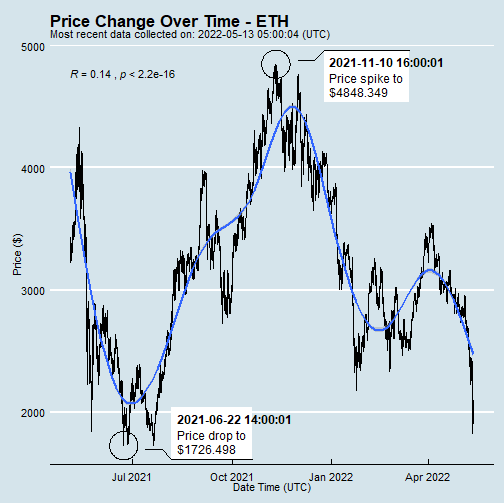
\includegraphics{pdf_document_files/figure-latex/unnamed-chunk-2-1.pdf}

\hypertarget{python-code-example}{%
\section{Python Code Example}\label{python-code-example}}

\begin{Shaded}
\begin{Highlighting}[]
\ImportTok{import}\NormalTok{ pandas }\ImportTok{as}\NormalTok{ pd}
\CommentTok{# Create the Python object from R}
\NormalTok{df }\OperatorTok{=}\NormalTok{ r.cryptodata}
\CommentTok{# Show the new Python dataframe}
\NormalTok{df}
\end{Highlighting}
\end{Shaded}

\begin{verbatim}
##         pair symbol  ask_1_price       date_time_utc
## 0     BTCUSD    BTC    26438.680 2020-12-29 06:00:01
## 1     ETHUSD    ETH      707.059 2020-12-29 06:00:01
## 2     BTCUSD    BTC    26479.250 2020-12-29 05:00:01
## 3     ETHUSD    ETH      704.794 2020-12-29 05:00:01
## 4     ETHUSD    ETH      699.948 2020-12-29 04:00:01
## ...      ...    ...          ...                 ...
## 5889  BTCUSD    BTC    11972.900 2020-08-10 06:03:50
## 5890  BTCUSD    BTC    11985.890 2020-08-10 05:03:48
## 5891  BTCUSD    BTC    11997.470 2020-08-10 04:32:55
## 5892  BTCUSD    BTC    10686.880                 NaT
## 5893  ETHUSD    ETH      357.844                 NaT
## 
## [5894 rows x 4 columns]
\end{verbatim}

\hypertarget{one-more-python-example}{%
\section{One more Python example}\label{one-more-python-example}}

The code below creates a new column \texttt{price\_percentile} that
specifies if the price for the row was in the upper or lower 50th
percentile of prices (BTC should be upper and ETH lower):

\begin{Shaded}
\begin{Highlighting}[]
\ImportTok{import}\NormalTok{ numpy }\ImportTok{as}\NormalTok{ np}
\CommentTok{# Create a new column based on the ask_1_price value:}
\NormalTok{df[}\StringTok{'price_percentile'}\NormalTok{] }\OperatorTok{=}\NormalTok{ np.where(df[}\StringTok{'ask_1_price'}\NormalTok{] }\OperatorTok{>} 
\NormalTok{                                  np.percentile(df[}\StringTok{'ask_1_price'}\NormalTok{], }\DecValTok{50}\NormalTok{),}
                            \StringTok{'upper 50th percentile of prices'}\NormalTok{, }
                            \StringTok{'lower 50th percentile of prices'}\NormalTok{)}
\CommentTok{# Show modified dataframe:}
\NormalTok{df[[}\StringTok{'symbol'}\NormalTok{, }\StringTok{'ask_1_price'}\NormalTok{, }\StringTok{'price_percentile'}\NormalTok{]]}
\end{Highlighting}
\end{Shaded}

\begin{verbatim}
##      symbol  ask_1_price                 price_percentile
## 0       BTC    26438.680  upper 50th percentile of prices
## 1       ETH      707.059  lower 50th percentile of prices
## 2       BTC    26479.250  upper 50th percentile of prices
## 3       ETH      704.794  lower 50th percentile of prices
## 4       ETH      699.948  lower 50th percentile of prices
## ...     ...          ...                              ...
## 5889    BTC    11972.900  upper 50th percentile of prices
## 5890    BTC    11985.890  upper 50th percentile of prices
## 5891    BTC    11997.470  upper 50th percentile of prices
## 5892    BTC    10686.880  upper 50th percentile of prices
## 5893    ETH      357.844  lower 50th percentile of prices
## 
## [5894 rows x 3 columns]
\end{verbatim}

\end{document}
